\documentclass{report}
\usepackage[utf8]{inputenc}
\usepackage{CJKutf8}
\usepackage{amsmath}
\usepackage{tikz-qtree}
\usepackage{pgfplots}
\usepackage{hyperref}
\usepackage{graphicx}
\usepackage{cases}
\usepackage{float}
\usetikzlibrary{trees}
\title{ネットワーク設計論レポート2}
\author{27019679 グレゴリウスブライアン}
\setlength{\parindent}{0pt}

\begin{document}
\begin{CJK}{UTF8}{min}
    \maketitle
    \section*{前書き}
    このレポートのすべてのグラフはpythonで生成され、添付されたnotebook(.ipynb)で記載されている。
    グラフの表現、描画はnetworkxライブラリーを使用している。また、アルゴリズム自体を説明すると記載されていない課題は
    ライブラリーのアルゴリズム関数を用いる場合がある(演習7の連結度を決定するための最小カットなど)

    また、このレポートで集合は「\{\}」だけでなく「[]」でも表記される。(プログラムとの互換性のため)
    \newpage
    \section*{演習7 問題1(グラフ基本)}

    \begin{figure}[!h]
        \centerline{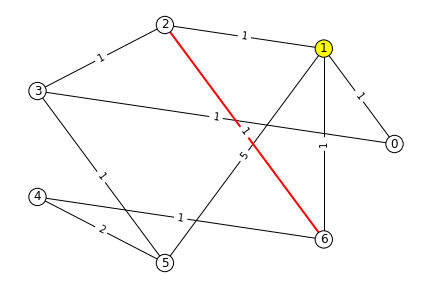
\includegraphics[width=0.8\textwidth]{data/1.png}}
        \caption{グラフの例}
    \end{figure}


    \begin{figure}[!h]
        \centerline{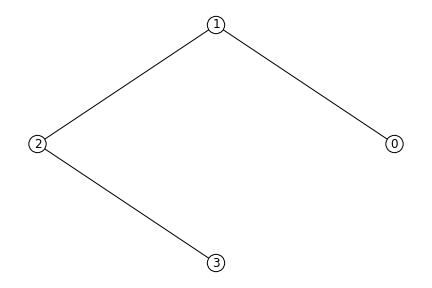
\includegraphics[width=0.8\textwidth]{data/2.png}}
        \caption{Figure 1 の部分グラフ例}
    \end{figure}


    \begin{figure}[!h]
        \centerline{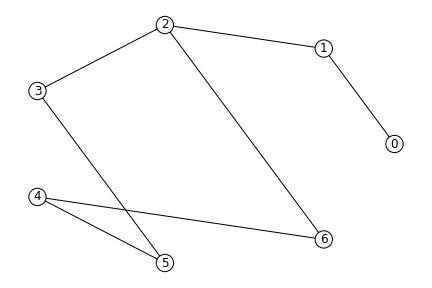
\includegraphics[width=0.8\textwidth]{data/3.png}}
        \caption{Figure 1 の全域部分グラフ例}
    \end{figure}

    \begin{figure}[!h]
        \centerline{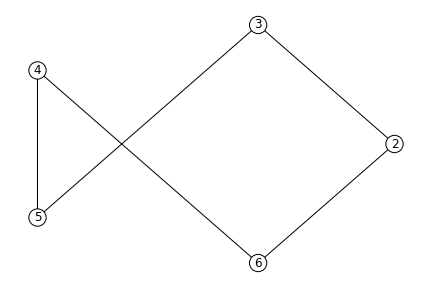
\includegraphics[width=0.8\textwidth]{data/4.png}}
        \caption{Figure 1 の頂点集合$[2,3,4,5,6]$で誘導される生成部分グラフ}
    \end{figure}

    \clearpage
    \section*{演習7 問題2(頂点部分集合のカットサイズ)}
    \begin{figure}[!h]
        \centerline{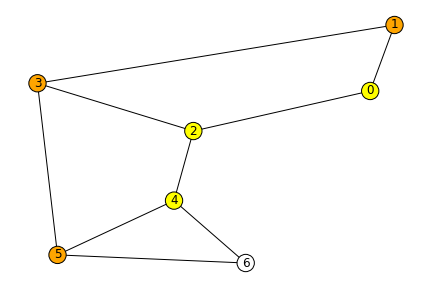
\includegraphics[width=0.8\textwidth]{data/5.png}}
        \caption{頂点集合$[0,2,4]$と$[1,3,5]$が$4$辺連結のグラフ}
    \end{figure}
    Figure 5 で示される黄色の頂点集合$[0,2,4]$とオレンジ色の頂点集合$[1,3,5]$のカットサイズが$4$である。そのうち一例のカットはFigure 6である。
    \begin{figure}[!h]
        \centerline{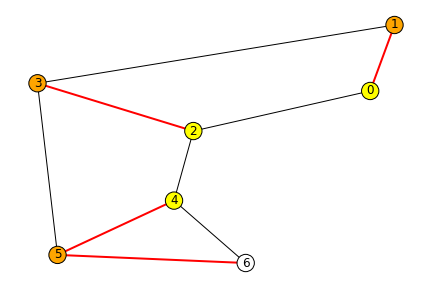
\includegraphics[width=0.8\textwidth]{data/6.png}}
        \caption{Figure 5 のカット例}
    \end{figure}

    \clearpage
    \section*{演習7 問題3(辺独立、点独立、辺素、内素)}
    \begin{figure}[!h]
        \centerline{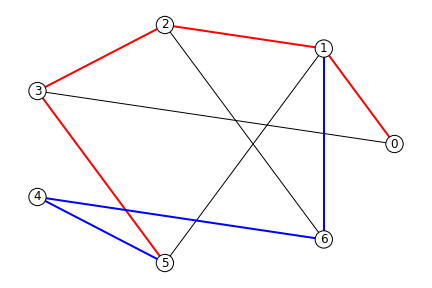
\includegraphics[width=0.8\textwidth]{data/7.png}}
        \caption{互いに辺独立な経路集合 $[0,1,2,3,5]$ (赤)と $[1,6,4,5]$ (青)}
    \end{figure}
    \begin{figure}[!h]
        \centerline{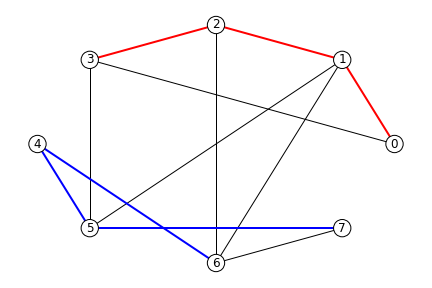
\includegraphics[width=0.8\textwidth]{data/8.png}}
        \caption{互いに点独立な経路集合 $[0,1,2,3]$ (赤)と $[6,4,5,7]$ (青)}
    \end{figure}
    \begin{figure}[!h]
        \centerline{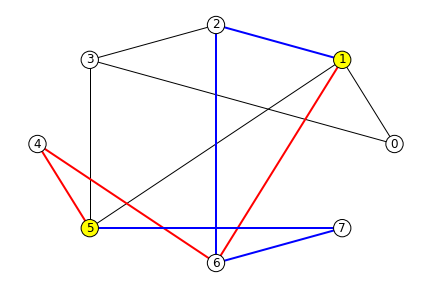
\includegraphics[width=0.8\textwidth]{data/9.png}}
        \caption{互いに辺素な経路集合 $[1,6,4,5]$ (赤)と $[1,2,6,7,5]$ (青)}
    \end{figure}
    \begin{figure}[!h]
        \centerline{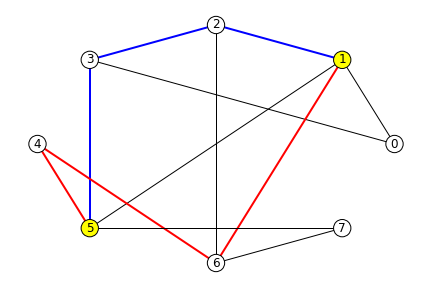
\includegraphics[width=0.8\textwidth]{data/10.png}}
        \caption{互いに内素な経路集合 $[1,6,4,5]$ (赤)と $[1,2,3,5]$ (青)}
    \end{figure}

    \clearpage
    \section*{演習7 問題4(頂点対の辺連結度)}
    \begin{figure}[!h]
        \centerline{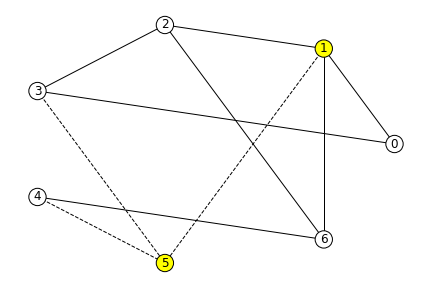
\includegraphics[width=0.8\textwidth]{data/11.png}}
        \caption{3辺連結の頂点対$(1,5)$とその最小カット(点線)}
    \end{figure}
    ただし、ここではすべての辺の容量は$1$であり、最小カットを決定するのにライブラリーの最大フロー・最小カット関数を用いた。

    \clearpage
    \section*{演習7 問題5(グラフの連結度)}
    \begin{figure}[!h]
        \centerline{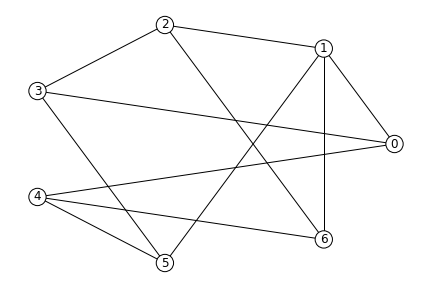
\includegraphics[width=0.8\textwidth]{data/12.png}}
        \caption{連結度3のグラフ}
    \end{figure}
    上記のグラフはすべての頂点対の最小カットは3である。したがって、これは連結度3のグラフの一例である。
    コードですべての頂点対の最小カットを調べている。

    \clearpage
    \section*{演習7問題6(頂点対の最大辺素経路)}
    \begin{figure}[!h]
        \centerline{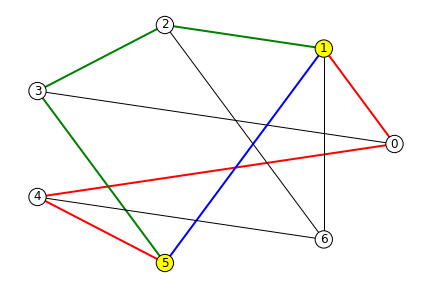
\includegraphics[width=0.8\textwidth]{data/13.png}}
        \caption{グラフと最大辺素経路集合}
    \end{figure}

    上記のグラフに対して、頂点対$[1,5]$の辺素な経路集合の経路数が$3$であり、
    それぞれ、$[1,0,4,5]$(赤)、$[1,5]$(青)、$[1,2,3,5]$(緑)である。
    そして、その同じサイズのカットは次通りである。
    \begin{figure}[!h]
        \centerline{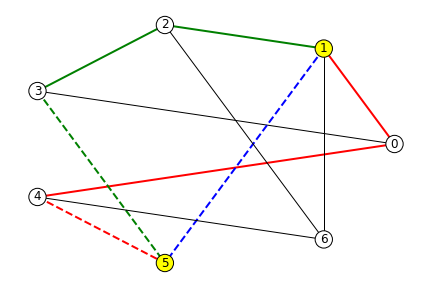
\includegraphics[width=0.8\textwidth]{data/14.png}}
        \caption{Figure 13のカット}
    \end{figure}


    \clearpage
    \section*{演習7問題7(NA辺連結度)}
    \begin{figure}[!h]
        \centerline{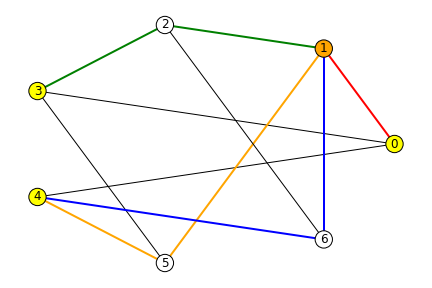
\includegraphics[width=0.8\textwidth]{data/15.png}}
        \caption{Node($1$)-to-Area($[ 0,3,4 ]$)連結度}
    \end{figure}
    上記の頂点$1$と領域$[0,3,4]$のNA辺連結は$4$であり、NA間の辺素経路をそれぞれの色で表せる。
    M
    \clearpage
    \section*{演習8 問題3(k辺連結保存))}
    Figure 12の2辺連結性保存を決めたい。コードでアルゴリズム自体を実装した。MA順序、辺順位決定の結果はFigure 16であり、
    Figure 16で得られた辺順位が1と2を取るとFigure 17である2辺連結性保存全域部分グラフができる。ただし、MA順序決定の過程は
    Figure 18で示され、辺順位決定の過程は Figure 19で示される(図の大きさの関係で結果が先に示す)。辺順位決定は逆順で行っていることに注意(コードが書きやすい)。
    \begin{figure}[!h]
        \centerline{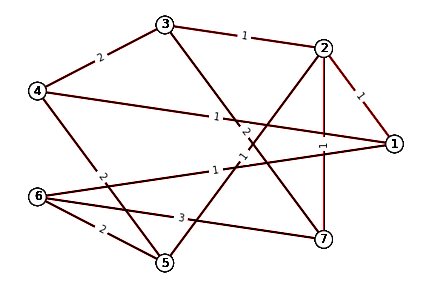
\includegraphics[width=0.8\textwidth]{data/ex-8-F-7.png}}
        \caption{MA順序、辺順位決定結果}
    \end{figure}

    \begin{figure}[!h]
        \centerline{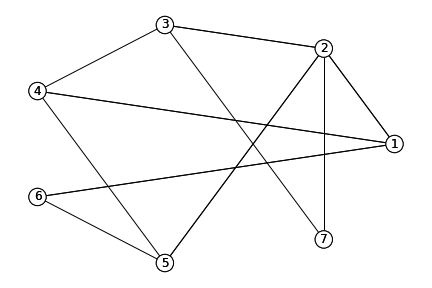
\includegraphics[width=0.8\textwidth]{data/ex-8-2S.png}}
        \caption{Figure 12の2辺連結性保存全域部分グラフ}
    \end{figure}

    \begin{figure}
        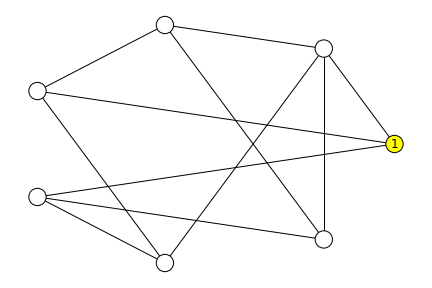
\includegraphics[width=.49\textwidth]{data/ex-8-NA-1.png}\hfill
        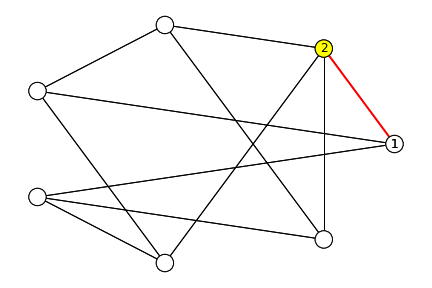
\includegraphics[width=.49\textwidth]{data/ex-8-NA-2.png}
        \\[\smallskipamount]
        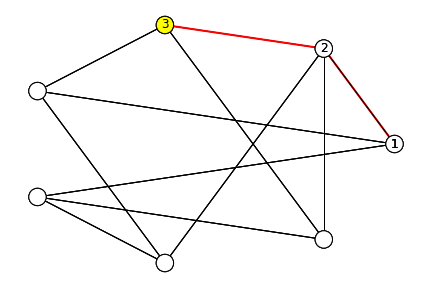
\includegraphics[width=.49\textwidth]{data/ex-8-NA-3.png}\hfill
        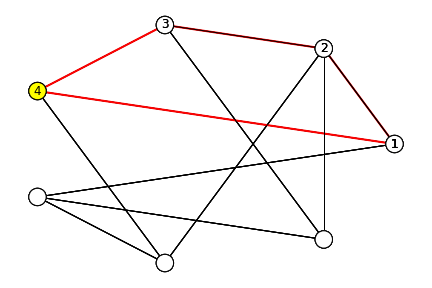
\includegraphics[width=.49\textwidth]{data/ex-8-NA-4.png}
        \\[\smallskipamount]
        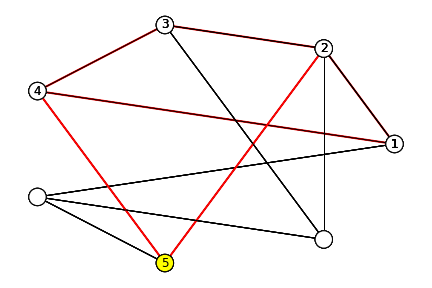
\includegraphics[width=.49\textwidth]{data/ex-8-NA-5.png}\hfill
        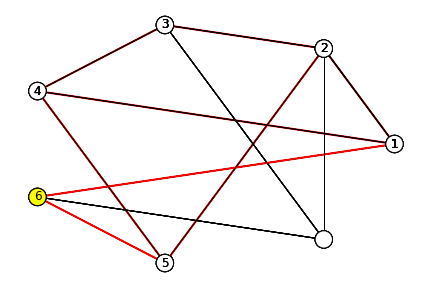
\includegraphics[width=.49\textwidth]{data/ex-8-NA-6.png}
        \\[\smallskipamount]
        \centerline{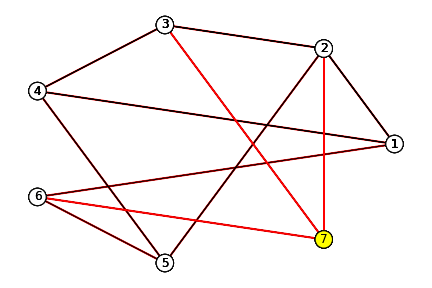
\includegraphics[width=.49\textwidth]{data/ex-8-NA-7.png}}
        \caption{MA順序決定}
    \end{figure}
    \begin{figure}
        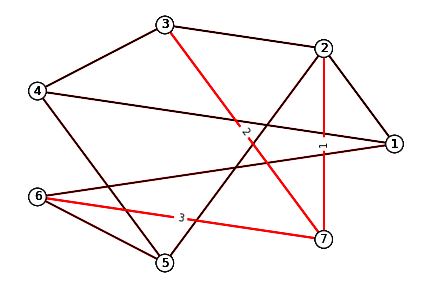
\includegraphics[width=.49\textwidth]{data/ex-8-F-1.png}\hfill
        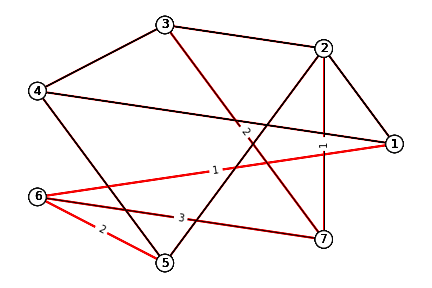
\includegraphics[width=.49\textwidth]{data/ex-8-F-2.png}
        \\[\smallskipamount]
        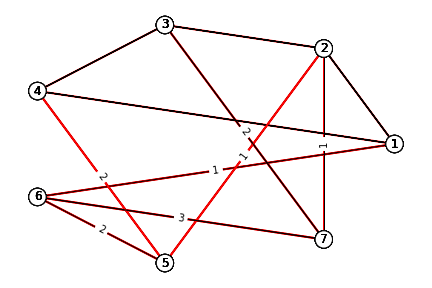
\includegraphics[width=.49\textwidth]{data/ex-8-F-3.png}\hfill
        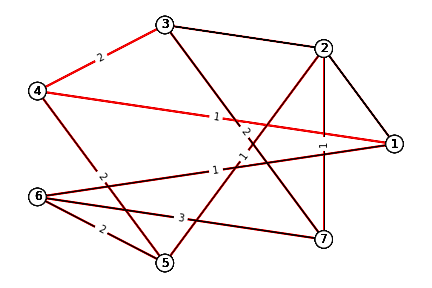
\includegraphics[width=.49\textwidth]{data/ex-8-F-4.png}
        \\[\smallskipamount]
        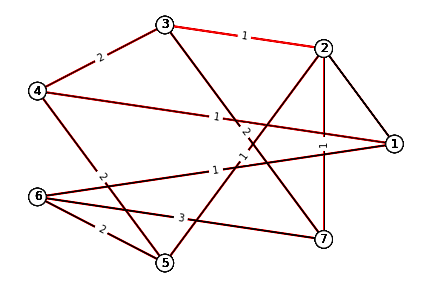
\includegraphics[width=.49\textwidth]{data/ex-8-F-5.png}\hfill
        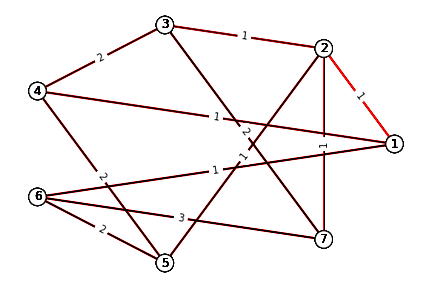
\includegraphics[width=.49\textwidth]{data/ex-8-F-6.png}
        \caption{辺の順位付け}
    \end{figure}

    \clearpage
    \section*{演習9問題1(辺連結分解)}
    Figure 1のグラフに対して辺連結分解を行う。見やすくするように、このグラフをレイアウト変更したグラフはFigure 20である。
    このグラフの連結度は2である。言い換えれば、2辺連結成分はグラフの頂点集合と等しい(Figure 20 黄色頂点)。そして、このグラフの3辺連結成分
    はFigure 21通りである。同じ色の頂点は同じ成分である。つまり、$V=[[0],[1,2,3,5,6],[4]]$。この方法はコード中のk\_edge\_decomposition(G,k)で実装され、
    k\_edge\_decomposition(G,3)は3辺連結成分を計算する形になっている。
    \begin{figure}[!h]
        \centerline{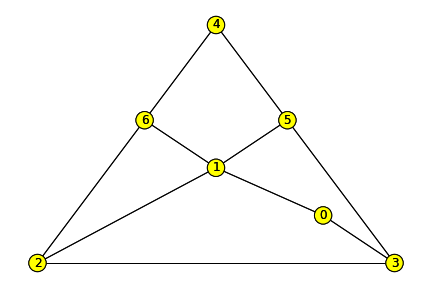
\includegraphics[width=0.7\textwidth]{data/ex-9-K-2.png}}
        \caption{Figure 1 の2辺連結成分}
    \end{figure}
    \begin{figure}[!h]
        \centerline{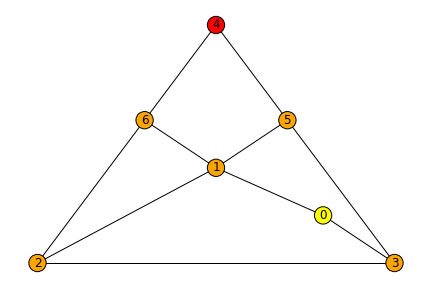
\includegraphics[width=0.7\textwidth]{data/ex-9-K-3.png}}
        \caption{Figure 1 の3辺連結成分}
    \end{figure}

    \clearpage
    \section*{演習9 問題3(木の辺付加)}
    連結性保存の時、2辺連結性保存のグラフがあるが、そのグラフの1辺連結性の保存を今回扱う木とする。深さ優先探索で
    葉に順序をつけたのがFigure 22である。ただし、探索は赤頂点から開始されるとする。そして、アルゴリズム通り辺を付加すれば
    Figure 23の2辺連結グラフになる。
    \begin{figure}[!h]
        \centerline{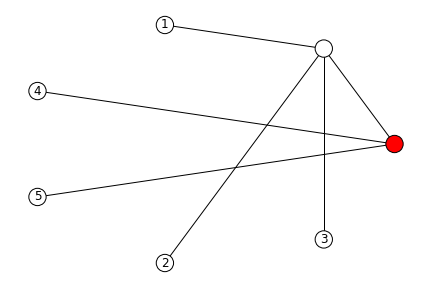
\includegraphics[width=0.8\textwidth]{data/ex9-def.png}}
        \caption{赤頂点から深さ優先探索、葉には順序をつける}
    \end{figure}
    \begin{figure}[!h]
        \centerline{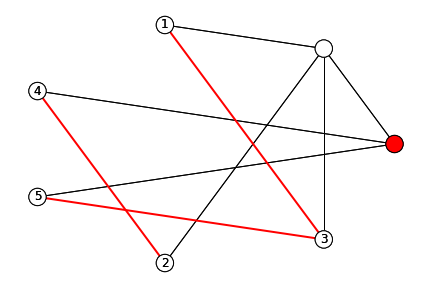
\includegraphics[width=0.8\textwidth]{data/ex9-T.png}}
        \caption{木の辺付加(付加した辺は赤)}
    \end{figure}


    \clearpage
    \section*{演習10問題1(直径増加抑制)}
    Figure 24のグラフは直径4のグラフである。どの2つの辺を消しても直径が4のままのように保護辺を決めたい。
    Figure 25がFigure 24の辺を頂点とするグラフであり。同時に2つの辺が切れたらグラフの直径が4より多くなったら辺を引く。
    それの頂点被覆(黄色頂点の集合)が保護辺の集合となり、Figure 26で示す。
    \begin{figure}[!h]
        \centerline{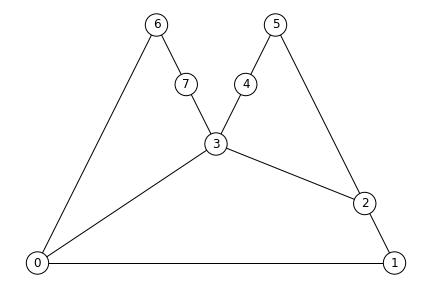
\includegraphics[width=0.8\textwidth]{data/ex10-1.png}}
        \caption{直径4のグラフ}
    \end{figure}
    \begin{figure}[!h]
        \centerline{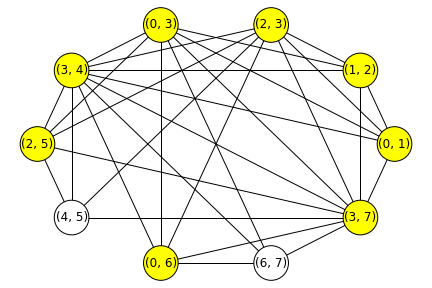
\includegraphics[width=0.8\textwidth]{data/ex10-2.png}}
        \caption{Figure 24の辺を頂点とするグラフ、黄色頂点は頂点被覆集合}
    \end{figure}
    \begin{figure}[!h]
        \centerline{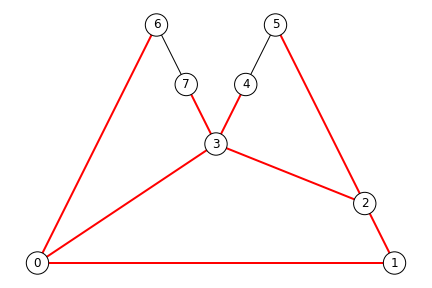
\includegraphics[width=0.8\textwidth]{data/ex10-3.png}}
        \caption{元のグラフの保護辺}
    \end{figure}

    \clearpage
    \section*{演習11問題1と2(ダイクストラ法最短路)}
    Figure 27のグラフに対して黄色頂点を根とする最短路木を作りたい。djikstraを用いた最短路木の探索
    はFigure 29で示される。ただし、Figure 29の黄色頂点は今探索中の頂点であり、オレンジ色の頂点は次に探索する頂点である。
    また、各頂点に記載されている数字は暫定最短路であり、赤いエッジは全体の最短路木になるエッジを示す。
    出来上がった最短路木はFigure 28で示される(頂点に付いている数字は根からの距離を示す)。
    \begin{figure}[!h]
        \centerline{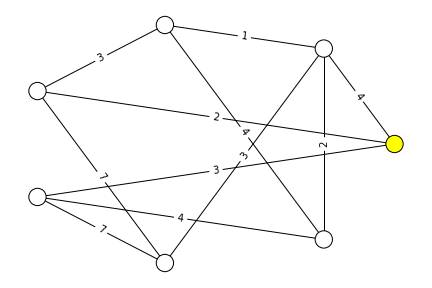
\includegraphics[width=0.8\textwidth]{data/ex-11-start.png}}
        \caption{重み付きグラフ}
    \end{figure}
    \begin{figure}[!h]
        \centerline{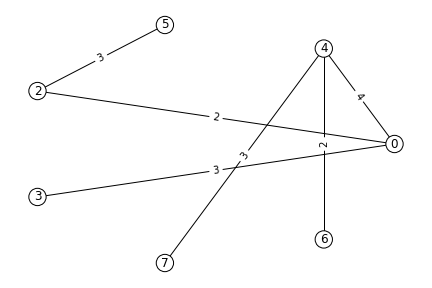
\includegraphics[width=0.8\textwidth]{data/ex-11-res.png}}
        \caption{Figure 27の最短路木}
    \end{figure}
    \begin{figure}
        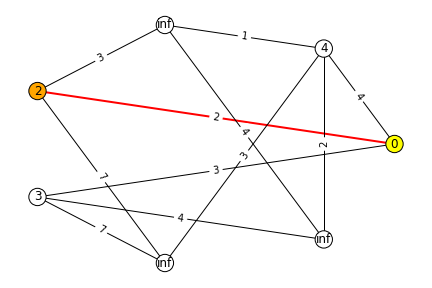
\includegraphics[width=.49\textwidth]{data/ex-11-D-1.png}\hfill
        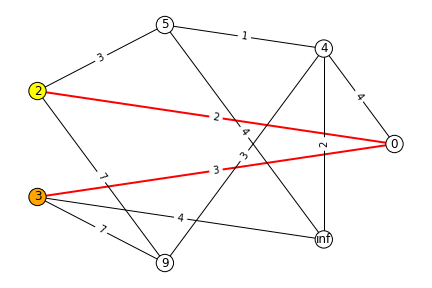
\includegraphics[width=.49\textwidth]{data/ex-11-D-2.png}
        \\[\smallskipamount]
        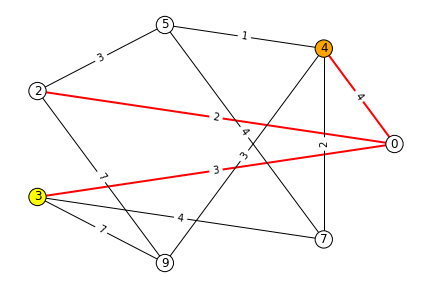
\includegraphics[width=.49\textwidth]{data/ex-11-D-3.png}\hfill
        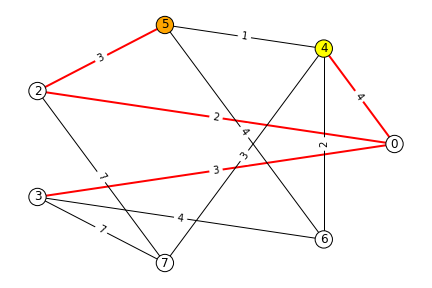
\includegraphics[width=.49\textwidth]{data/ex-11-D-4.png}
        \\[\smallskipamount]
        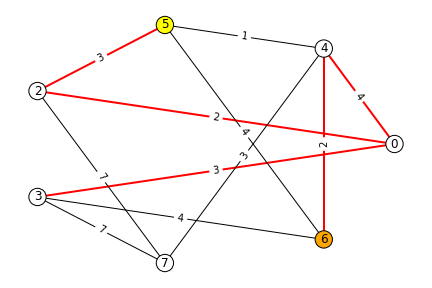
\includegraphics[width=.49\textwidth]{data/ex-11-D-5.png}\hfill
        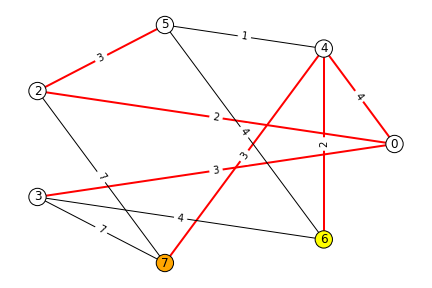
\includegraphics[width=.49\textwidth]{data/ex-11-D-6.png}
        \\[\smallskipamount]
        \caption{djikstra最短路過程}
    \end{figure}


    \clearpage
    \section*{演習11問題5(最大フロー)}
    ソースノードからシンクノードのパス有無を探すのにBFSを用いた。BFSも最大フローアルゴリズムも添付した.ipynbにゼロから実施した。
    Figure 30のグラフに対して0から3の最大フローを求める。その最大フローはFigure 31で示され、最大フローは47であることが分かる。
    最大フローを求める残余ネットワークの過程はFigure 32である。ここで、矢先に近い数字はその辺の容量である。
    \begin{figure}[!h]
        \centerline{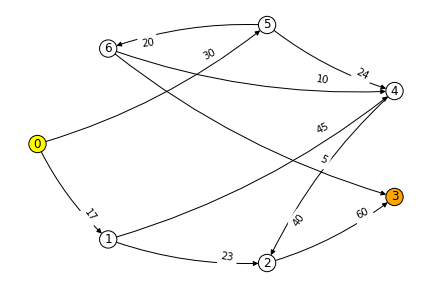
\includegraphics[width=0.8\textwidth]{data/ex11-MF-start.png}}
        \caption{容量付き有向グラフ}
    \end{figure}
    \begin{figure}[!h]
        \centerline{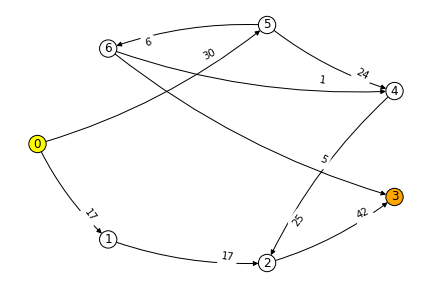
\includegraphics[width=0.8\textwidth]{data/ex11-MF-res.png}}
        \caption{Figure 30の最大フロー}
    \end{figure}
    \begin{figure}
        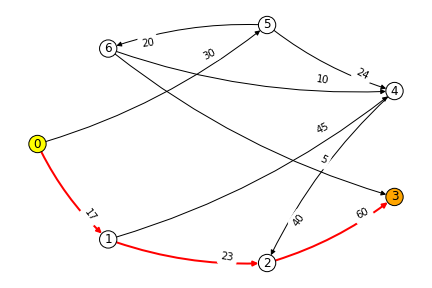
\includegraphics[width=.49\textwidth]{data/ex11-MF-1.png}\hfill
        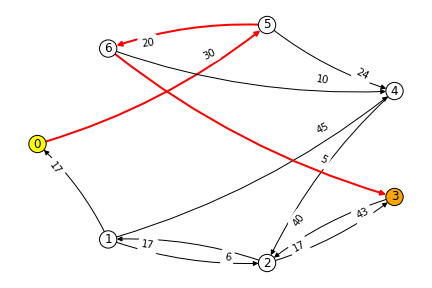
\includegraphics[width=.49\textwidth]{data/ex11-MF-2.png}
        \\[\smallskipamount]
        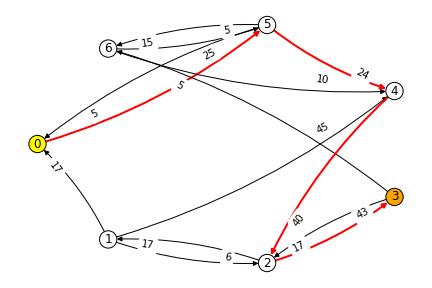
\includegraphics[width=.49\textwidth]{data/ex11-MF-3.png}\hfill
        \includegraphics[width=.49\textwidth]{data/ex11-MF-4.png}
        \caption{Ford-Fulkerson最大フロー過程}
    \end{figure}

    \clearpage
    \section*{演習11問題5(最大フロー)}
    Figure 33は容量とコスト付きの有向グラフであり、最大フローを計算したらFigure 34になる。
    しかし、Figure 35のように最大フローを求めたあとの残余グラフにはシンクノードにおいて負閉路が存在する。
    この閉路消したあとの最大フロー最小コストグラフはFigure 36である。

    \begin{figure}[!h]
        \centerline{\includegraphics[width=0.8\textwidth]{data/ex12-MF-start.png}}
        \caption{容量とコスト付き有向グラフ}
    \end{figure}
    \begin{figure}[!h]
        \centerline{\includegraphics[width=0.8\textwidth]{data/ex12-MF-flow-start.png}}
        \caption{初期最大フロー}
    \end{figure}
    \begin{figure}[!h]
        \centerline{\includegraphics[width=0.8\textwidth]{data/ex12-MF-1.png}}
        \caption{残余グラフに負閉路存在}
    \end{figure}
    \begin{figure}[!h]
        \centerline{\includegraphics[width=0.8\textwidth]{data/ex12-MF-flow-result.png}}
        \caption{最小コスト最大フロー}
    \end{figure}
\end{CJK}



\end{document}
